% !TeX root = ./jvk-blatt4.tex
\excercise{Shapes}
\begin{enumerate}
    \item Passe die Main Operation an die Aufgabe an. Verwende \lstinline{Sheet4Task2}. Verifier brauchst du nicht setzen, weil es in dieser Aufgabe keinen gibt.
    \item Zeichne, mithilfe des \lstinline{PlayfieldModifiers}, einen Smiley auf das Feld.
    \\ 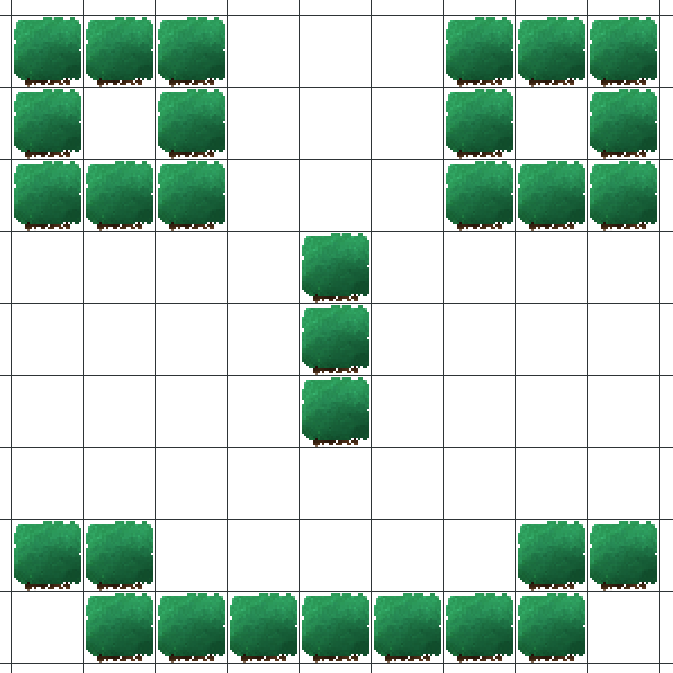
\includegraphics[width=\linewidth]{./figures/smily.png}
    \item Zeichne den Smiley mithilfe von Shapes. Du kannst dafür z.B. das Pixel Shape verwenden.
    \item Erstelle eine eigene Shape-klasse für Smilies und geb ihr einen Namen.
    \begin{Infobox}[Eclipse Class wizard]
    Wenn du im Package Explorer von Eclipse einen Rechtsklick machst, gibt es die Option new.
    Damit bekommst du ein kleines Menü an die Hand, um zum Beispiel eine Klasse zu erstellen.
    \end{Infobox}
    \item Füge das Interface Shape hinzu.
    \begin{lstlisting}[title=Interface Syntax,frame=ltr]
        class <ClassName> implements <InterfaceName>
        {
            /...
    \end{lstlisting}
    \begin{Infobox}[Interface]
        Interfaces werden auch als Verträge bezeichnet.
Wenn wir das Interface Shape hinzufügen, dann gehen wir einen Vertrag ein, dass wir ein Shape bauen.
Das heißt jeder kann unser Shape wie jedes andere Shape verwenden.
Damit das geht, müssen wir aber jede Operation haben, die auch im Interface verwendet wird.
Das machen wir, indem wir die Operation (mit dem gleichen Namen, Parametern und Modifern) bei uns hereinschreiben und davor (am besten in eine eigene Zeile) \lstinline{@Override}.
    \end{Infobox}    
    \item Implementiere den Konstruktor und baue darin das Smiley-shape zusammen. So wie du es in c) gemacht hast.
    \item Ein Shape muss eine ganz bestimmte Operation von Interface überschreiben, nämlich \lstinline{public Iterator<Position> iterator()}.
    Darin brauchen wir aber das Shape die wir vorhin bereits erstellt haben.
    Das steht aber in einer Variable vom Konstruktor.
    Die Lösung ist einfach: Wir ziehen die Variable aus dem Konstruktor, direkt in die Klasse.
    Wie bei den Operationen schreiben wir auch hier einfach mal ein  \lstinline{modifier} davor. Diesmal aber \lstinline{private}.
    Nun kann jede Operation und jeder Konstruktor dieselbe Variable verwenden.

    Wir wollen jetzt aber nicht einen eigenen Iterator schreiben oder kreieren. Also geben wir einfach zurück, was die Iterator-funktion des Pixel-shape uns zurückgibt.
\item Wie eine Operation kann auch ein Konstruktor Parameter haben.
Erstelle einen oder mehrere, mit denen du eine Position mitgeben kannst, an der das Smiley gezeichnet wird
und Zeichen ein paar an verschiedenen Positionen.
\end{enumerate}

\newpage
